Los autómatas regulares fueron introducidos por Huffman \cite{huffman} como
 herramientas para reconocer palabras de largo finito.
Pero para representar las ejecuciones de un sistema se necesita trabajar con palabras de largo infinito.
Para esto Büchi introdujo el concepto de Autómatas de Büchi (NBA) \cite{buchi}.
Estos son una variante de los autómatas
 regulares utilizados para reconocer palabras de largo infinito.

%Para verificar si un sistema $TS$ dado satisface una determinada propiedad se trabaja con el autómata de
% Büchi $\mathcal{A}$, que representa los "bad traces" de la propiedad ($\mathcal{A}$ reconoce el complemento
% de la propiedad a verificar). Se realiza el producto entre $\mathcal{A}$ y $TS$ y mediante un análisis del
% grafo se determina si $TS \models P$.


\section{Lenguajes \textit{omega}-regulares}
Llamamos lenguajes regulares a los lenguajes que se pueden representar mediante expresiones regulares.
Las palabras de estos lenguajes tienen largo finito.
 %, es decir secuencias de símbolos de largo finito.
 En cambio si queremos tratar con palabras de largo infinito necesitaremos una clase distinta de
 lenguajes, asociados con una clase distinta de expresiones. Esta nueva clase de lenguajes se denomina
 lenguajes \textit{omega}-regulares.
 
%Una palabra infinita sobre el alfabeto $\Sigma$ es una secuencia de símbolos pertenecientes a $\Sigma$.
Utilizaremos la letra griega $\omega$ (\textit{omega}) para denotar la repetición infinita,
 por ejemplo $a^\omega$ es la palabra
 infinita que contiene sólo símbolos $a$.\footnote{Notar que $a^*$ representa un lenguaje, es el conjunto de todas las palabras finitas que contienen únicamente el símbolo $a$, mientras que $a^\omega$ representa
 solamente una palabra.}
 
Llamamos $\Sigma^\omega$ al conjunto de todas las palabras infinitas sobre $\Sigma$.
 Cualquier subconjunto de $\Sigma^\omega$ es un lenguaje de palabras infinitas.

\begin{definicion}
Expresión $\omega$-regular.\\
Una expresión $\omega$-regular $G$ sobre el alfabeto $\Sigma$ tiene la siguiente forma
\[ G = E_1.F_1^\omega + ... + E_n.F_n^\omega \]
donde $n \geq 1$ y $E_1, ..., E_n, F_1, ..., F_n$ son expresiones regulares sobre $\Sigma$ tales que
 $\varepsilon \not\in L(F_i)$, siendo $L(F_i)$ el lenguaje representado por la expresión regular $F_i$.
\end{definicion}

Un lenguaje $\omega$-regular, análogamente a los regulares, es un lenguaje que se puede representar
mediante una expresión $\omega$-regular.


 
 
\paragraph{Ejemplo.}
Considerando el NBA de la figura \ref{fig:nba} sobre el alfabeto $\{ A, B, C \}$.\\

\begin{figure}[hbtp]
\begin{center}
\caption{Ejemplo de Autómata de Büchi}
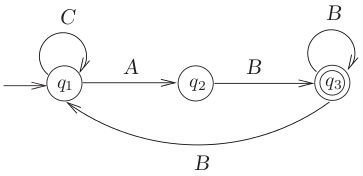
\includegraphics[width=0.7\textwidth]{buchi/imagenes/ejemplo4_28.png}
\label{fig:nba}
\end{center}
\end{figure}

El lenguaje aceptado por el NBA está dado por la expresión regular
\[ C^*AB(B^+ + BC^*AB)^\omega \]
 
\section{Autómata de Büchi Generalizado}
En este trabajo se utiliza una variante de los NBA, el Autómata de Buchi Generalizado (GNBA).
La estructura de los GNBAs es muy similar a la de los NBAs, varía sólo en el conjunto de aceptación.
En lugar de este contiene un conjunto F cuyos elementos son los conjuntos de aceptación $F_i$.
El criterio de aceptación en estos autómatas es visitar infinitas veces todos los conjuntos de
 aceptación $F_i$.

\begin{definicion}
Autómatas de Büchi Generalizado.\\
Los Autómatas de Büchi Generalizado (GNBA) consisten en una tupla $\mathcal{G} = (\text{Q}, \Sigma, \delta, \text{Q}_0, \mathcal{F})$, donde: $\text{Q}$, $\Sigma$, $\delta$ y $\text{Q}_0$ se definen
igual que en los NBA mientras que $\mathcal{F} \subseteq 2^Q$ es el conjunto de aceptación.
\end{definicion}

El lenguaje aceptado por un GNBA $\mathcal{G}$ consiste en todas las palabras que pasan infinitas
 veces por todos los conjuntos de aceptación.

Más formalmente, dado un GNBA $\mathcal{G} = (\text{Q}, \Sigma, \delta, \text{Q}_0, \mathcal{F})$ y
 una secuencia infinita de estados $q_0 q_1 q_2 q_3 ...$, esta es aceptada por $\mathcal{G}$ si
\[ \forall \text{F} \in \mathcal{F}, \exists \text{ infinitas } j \in \mathbb{N} \text{ tal que } q_j \in F \]

 
\paragraph{Ejemplo.}
En la figura \ref{fig:seccion_critica} se muestra un GNBA sobre el alfabeto $2^{AP}$
 donde $AP = \{ crit_1, crit_2 \}$ y los conjuntos de aceptación
 $F_1 = \{ q_1 \}$ y $F_2 = \{ q_2 \}$.

\begin{figure}[hbtp]
\begin{center}
\caption{GNBA para sección crítica}
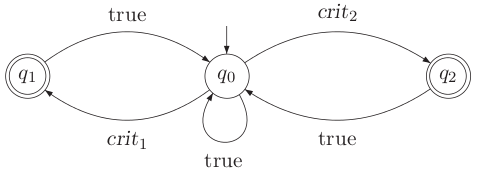
\includegraphics[width=0.7\textwidth]{buchi/imagenes/ejemplo4_53.png}
\label{fig:seccion_critica}
\end{center}
\end{figure}

El lenguaje aceptado es la propiedad que contiene todas las palabras infinitas tal que $crit_1$ y 
$crit_2$ ocurren infinitas veces.
Este GNBA representa la propiedad de que ninguno de los procesos quede infinitamente
 esperando para ingresar a la sección crítica.
